\documentclass{standalone}
\usepackage{ tikz }
\usepackage{ xparse }
\usepackage{../../../macros}
\usetikzlibrary{shapes}

\begin{document}
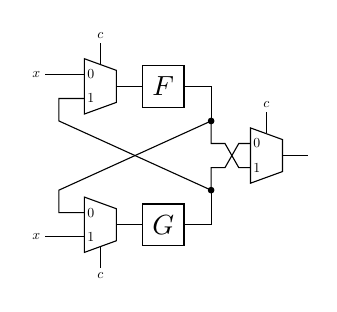
\begin{tikzpicture}[yscale=-1,x=1em,y=1.25em]
        
    \draw (-0.5,0.15) -- (0.9,0.15);  
    \node [draw,trapezium,trapezium left angle=70,trapezium right angle=70,rotate=-90,minimum width = 2em, minimum height =1em] at (1.5,0.5) {};
    \node [scale=0.5] at (1.15,0.15) {$0$};
    \node [scale=0.5] at (1.15,0.85) {$1$};
    \draw (1.5,-0.75) -- (1.5,-0.14);
    \node [scale=0.5, anchor=south] at (1.5, -0.75) {$c$};
    \draw (2.1,0.5) -- (3,0.5);
    \node [draw, minimum width=1.5em, minimum height=1.5em, anchor=west] at (3,0.5) {$F$};
    \draw (4.5,0.5) -- (5.5,0.5) -- (5.5,1.5);
    \filldraw (5.5,1.5) circle (1pt);
    \draw (5.5,1.5) -- (5.5,2.15) -- (6,2.15) -- (6.5,2.85) -- (6.9,2.85);
    \draw (5.5,1.5) -- (0,3.5) -- (0,4.15) -- (0.9,4.15);
    \node [draw,trapezium,trapezium left angle=70,trapezium right angle=70,rotate=-90,minimum width = 2em, minimum height =1em] at (1.5,4.5) {};
    \node [scale=0.5] at (1.15,4.15) {$0$};
    \node [scale=0.5] at (1.15,4.85) {$1$};
    \draw (-0.5,4.85) -- (0.9,4.85);
    \draw (1.5,5.75) -- (1.5,5.14);
    \node [scale=0.5, anchor=north] at (1.5, 5.75) {$c$};
    \draw (2.1,4.5) -- (3,4.5);
    \node [draw, minimum width=1.5em, minimum height=1.5em, anchor=west] at (3,4.5) {$G$};
    \draw (4.5,4.5) -- (5.5,4.5) -- (5.5,3.5);
    \filldraw (5.5,3.5) circle (1pt);
    \draw (5.5,3.5) -- (0,1.5) -- (0,0.85) -- (0.9,0.85);
    \draw (5.5,3.5) -- (5.5,2.85) -- (6,2.85) -- (6.5,2.15) -- (6.9,2.15);
    \node [draw,trapezium,trapezium left angle=70,trapezium right angle=70,rotate=-90,minimum width = 2em, minimum height =1em] at (7.5,2.5) {};
    \node [scale=0.5] at (7.15,2.15) {$0$};
    \node [scale=0.5] at (7.15,2.85) {$1$};
    \draw (8.1,2.5) -- (9,2.5);
    \draw (7.5,1.25) -- (7.5,1.86);
    \node [scale=0.5, anchor=south] at (7.5, 1.25) {$c$};
    \node [scale=0.5, anchor=east] at (-0.5, 0.15) {$x$};
    \node [scale=0.5, anchor=east] at (-0.5, 4.85) {$x$};
\end{tikzpicture}
\end{document}